\section{Результаты}
\label{sec:results}

\subsection{HAR-RV бенчмарк}

Все эконометрические и ML-модели в данной работе используют единую
реализацию метрик качества (\texttt{src/models/metrics.py}) с канонической
формулой QLIKE по Patton~\cite{Patton2011}. Это обеспечивает корректность
попарного сравнения, ранее затруднённого расхождением формул в разных
модельных модулях.
Дополнительно все sentiment- и attention-признаки используются
с лагом~1 (значение, известное к концу предыдущего торгового дня),
что исключает потенциальный data leakage при прогнозе $\mathrm{RV}_t$.

Результаты оценки HAR-log модели на золоте (GLDRUB\_TOM) методом
расширяющегося окна (обучение 60\%, тест 40\%, $n_{\text{test}} = 773$
дня для золота и $n_{\text{test}} = 654$ для серебра) представлены
в таблице~\ref{tab:har_results}.

\begin{table}[h!]
\centering
\caption{Метрики HAR-log модели (expanding window OOS)}
\label{tab:har_results}
\begin{tabular}{llrrrr}
\hline
Инструмент & Спецификация & MAE & RMSE & $R^2_{\mathrm{OOS}}$ & QLIKE \\
\hline
GLDRUB\_TOM & HAR-log & 0{,}674 & 0{,}869 & 0{,}177 & 0{,}628 \\
SLVRUB\_TOM & HAR-log & 0{,}838 & 1{,}060 & 0{,}377 & 0{,}979 \\
\hline
\end{tabular}
\end{table}

Модель HAR-log демонстрирует положительный $R^2_{\mathrm{OOS}}$
для обоих инструментов: $0{,}177$ для золота и $0{,}377$ для серебра,
что означает превосходство над наивным прогнозом средним.
Оценка МНК на полной выборке даёт $R^2 = 0{,}606$ (золото) и $0{,}550$ (серебро),
что типично для HAR-моделей на дневных данных.

Для золота (GLDRUB\_TOM, $n=1\,931$):
$\hat\alpha=-0{,}524$, $\hat\beta_d = 0{,}143$, $\hat\beta_w = 0{,}353$, $\hat\beta_m = 0{,}451$.
Для серебра (SLVRUB\_TOM, $n=1\,635$):
$\hat\alpha=-1{,}039$, $\hat\beta_d = 0{,}171$, $\hat\beta_w = 0{,}411$, $\hat\beta_m = 0{,}296$.
Выполнение неравенства $\hat\beta_m > \hat\beta_w > \hat\beta_d$
для золота соответствует теоретическим предсказаниям HAR-модели
об убывании скорости адаптации участников с более длинным горизонтом.

\subsection{HAR-log-S с многоисточниковым sentiment-вектором}

Модель HAR-log-S расширяет HAR-log дневным и недельным значениями
взвешенного индекса $S_t^{\text{comb}}$~(\ref{eq:sent_comb}),
объединяющего RSS-, GDELT- и Telegram-сигналы.
В таблице~\ref{tab:har_s_results} приведено сравнение спецификации
со включённым sentiment с базовой HAR-log.

\begin{table}[h!]
\centering
\caption{HAR-log vs HAR-log-S (sentiment\_combined, лаг~1)}
\label{tab:har_s_results}
\begin{tabular}{llrrrr}
\hline
Инструмент & Модель & MAE & RMSE & $R^2_{\mathrm{OOS}}$ & QLIKE \\
\hline
GLDRUB\_TOM & HAR-log   & 0{,}674 & 0{,}869 & 0{,}177 & 0{,}628 \\
GLDRUB\_TOM & HAR-log-S & \textbf{0{,}672} & \textbf{0{,}868} & \textbf{0{,}180} & \textbf{0{,}626} \\
SLVRUB\_TOM & HAR-log   & 0{,}838 & 1{,}060 & \textbf{0{,}377} & \textbf{0{,}979} \\
SLVRUB\_TOM & HAR-log-S & \textbf{0{,}834} & 1{,}060 & 0{,}376 & 1{,}022 \\
\hline
\end{tabular}
\end{table}

На золоте HAR-log-S улучшает все четыре метрики, хотя прирост невелик
(MAE снижается на 0{,}3\%, $R^2_{\mathrm{OOS}}$ растёт с 0{,}177 до 0{,}180).
На серебре наблюдается смешанный эффект: MAE снижается с 0{,}838 до 0{,}834,
однако QLIKE ухудшается с 0{,}979 до 1{,}022, а $R^2_{\mathrm{OOS}}$
остаётся практически неизменным.
Тест Диболда--Мариано~\cite{Diebold1995} (раздел~\ref{sec:dm}) показывает,
что улучшение по MAE значимо лишь на уровне 10\%
($p=0{,}078$ для золота, $p=0{,}070$ для серебра),
а на серебре по QLIKE sentiment даже статистически значимо \textit{ухудшает}
прогноз ($p<0{,}001$).
Это согласуется с интерпретацией: добавление шумного многоисточникового
sentiment может незначительно улучшать центр распределения ошибки (MAE),
но повышать дисперсию по краям (QLIKE).

\subsection{Ablation: вклад отдельных sentiment-источников}
\label{sec:har_ablation}

Для понимания роли каждого источника проведено ablation-исследование
HAR-log-S с подстановкой одного источника вместо взвешенного индекса
(таблица~\ref{tab:har_ablation}).

\begin{table}[h!]
\centering
\caption{HAR-log-S ablation: вклад каждого sentiment/attention-источника}
\label{tab:har_ablation}
\small
\begin{tabular}{llrrrr}
\hline
Инструмент & Источник $S_t$ & MAE & RMSE & $R^2_{\mathrm{OOS}}$ & QLIKE \\
\hline
GLDRUB\_TOM & HAR-log (без $S$)   & 0{,}6744 & 0{,}8694 & 0{,}1773 & 0{,}6281 \\
GLDRUB\_TOM & sentiment\_combined & \textbf{0{,}6723} & \textbf{0{,}8682} & \textbf{0{,}1795} & 0{,}6261 \\
GLDRUB\_TOM & sentiment\_score (RSS) & 0{,}6744 & 0{,}8694 & 0{,}1773 & 0{,}6281 \\
GLDRUB\_TOM & sentiment\_gdelt     & 0{,}6756 & 0{,}8700 & 0{,}1760 & 0{,}6267 \\
GLDRUB\_TOM & tg\_score (Telegram) & 0{,}6725 & 0{,}8689 & 0{,}1781 & 0{,}6364 \\
GLDRUB\_TOM & attention\_google    & 0{,}6878 & 0{,}8815 & 0{,}1541 & \textbf{0{,}5905} \\
\hline
SLVRUB\_TOM & HAR-log (без $S$)   & 0{,}8383 & 1{,}0596 & 0{,}3765 & 0{,}9790 \\
SLVRUB\_TOM & sentiment\_combined & 0{,}8342 & 1{,}0599 & 0{,}3762 & 1{,}0216 \\
SLVRUB\_TOM & sentiment\_score (RSS) & 0{,}8383 & 1{,}0596 & 0{,}3765 & 0{,}9790 \\
SLVRUB\_TOM & sentiment\_gdelt    & 0{,}8400 & 1{,}0610 & 0{,}3749 & 0{,}9765 \\
SLVRUB\_TOM & tg\_score (Telegram) & \textbf{0{,}8352} & 1{,}0621 & 0{,}3736 & 1{,}0364 \\
SLVRUB\_TOM & attention\_google   & 0{,}8466 & \textbf{1{,}0585} & \textbf{0{,}3778} & \textbf{0{,}9729} \\
\hline
\end{tabular}
\end{table}

Ключевые наблюдения:
\begin{enumerate}
    \item \textbf{RSS даёт нулевой вклад.} Замена на чистый RSS-индекс
          приводит к метрикам, побитово совпадающим с HAR-log без sentiment.
          Это указывает, что в текущей версии \texttt{rss\_news.csv}
          NLP-агрегация даёт постоянное (нулевое) значение для большинства
          торговых дней, что нейтрализует регрессор.
    \item \textbf{Для золота сильнейший источник~--- взвешенный комбинированный
          индекс} (RSS+GDELT+Telegram), что подтверждает гипотезу о
          диверсификации источников.
    \item \textbf{Для серебра доминирует \texttt{attention\_google}}~---
          индекс поисковой активности Google Trends, дающий
          \textit{лучший} $R^2_{\mathrm{OOS}}$ и QLIKE на этом инструменте.
          Это согласуется с теоретической работой
          Да, Энгельберг и Гао~\cite{Da2011} об индексе внимания розничных
          инвесторов как самостоятельной предиктивной переменной,
          особенно значимой для активов с высокой долей розничного спроса.
    \item Telegram-индекс полезен по MAE на обоих инструментах,
          но не улучшает QLIKE.
\end{enumerate}

\subsection{kNN на пространстве информационных состояний}

По методологии Halousková и Lyócsa~\cite{Halouskova2025}
реализован kNN-прогнозировщик: для каждого тестового дня $t$
находятся $k$ исторически ближайших дней в нормированном пространстве
признаков (HAR-лаги $+$ sentiment-вектор из 6 переменных).
Сходство вычисляется как обратное расстояние (inverse-distance kernel):
\[
  \mathrm{sim}(t, s) = \frac{1}{1+\|\mathbf{h}_t - \mathbf{h}_s\|} +
                       \frac{w_s}{1+\|\mathbf{s}_t - \mathbf{s}_s\|},
  \quad w_s = 1{,}0,
\]
прогноз~--- взвешенное среднее $\log\mathrm{RV}$ соседей.
Оптимальное $k$ подбирается по обучающей выборке с использованием
тех же sentiment-данных с лагом~1.
После исправления QLIKE-метрики и фикса leakage оптимумы
сместились в сторону больших значений: $k^* = 75$ (GLDRUB\_TOM)
и $k^* = 30$ (SLVRUB\_TOM).
Метрики приведены в таблице~\ref{tab:knn_results}.

\begin{table}[h!]
\centering
\caption{kNN с оптимальным $k$ (после фикса QLIKE и sentiment-лага)}
\label{tab:knn_results}
\begin{tabular}{llrrrr}
\hline
Инструмент & Модель & MAE & RMSE & $R^2_{\mathrm{OOS}}$ & QLIKE \\
\hline
GLDRUB\_TOM & kNN ($k=75$) & 0{,}671 & 0{,}877 & 0{,}163 & 0{,}683 \\
SLVRUB\_TOM & kNN ($k=30$) & 0{,}859 & 1{,}086 & 0{,}345 & 1{,}167 \\
\hline
\end{tabular}
\end{table}

\subsection{XGBoost}

Модель градиентного бустинга XGBoost~\cite{Chen2016} обучается на
расширенном наборе признаков: HAR-лаги, дополнительные лаги
$\mathrm{RV}_{t-k}$ ($k=2,\ldots,5$) и sentiment-вектор
(\texttt{sentiment\_combined}, \texttt{sentiment\_gdelt},
\texttt{tg\_score}, \texttt{attention\_google})
с лагом~1 для совместимости с настройкой HAR-log-S.
Гиперпараметры: глубина деревьев~4, скорость обучения~0{,}05,
300~деревьев, $L_1$-регуляризация~0{,}1.
Разбиение обучения/теста~--- 60/40 по времени без перемешивания
(в отличие от expanding-window для HAR и kNN, что отдельно отмечено
в обсуждении методологии).

Результаты XGBoost на корректно подготовленных данных
(таблица~\ref{tab:xgb_results}, требуется запуск
\texttt{python3 -m src.models.ml\_models}; библиотека
\texttt{xgboost} устанавливается отдельно):

\begin{table}[h!]
\centering
\caption{XGBoost на расширенном наборе признаков с лагированным sentiment}
\label{tab:xgb_results}
\begin{tabular}{llrrrr}
\hline
Инструмент & Модель & MAE & RMSE & $R^2_{\mathrm{OOS}}$ & QLIKE \\
\hline
GLDRUB\_TOM & XGBoost & 0{,}725 & 0{,}924 & 0{,}070 & 0{,}627 \\
SLVRUB\_TOM & XGBoost & 0{,}879 & 1{,}119 & 0{,}305 & 1{,}237 \\
\hline
\end{tabular}
\end{table}

Анализ важности признаков (feature importance) по методу средней прибыли деревьев
показывает доминирование HAR-лагов над sentiment-признаками.
Для GLDRUB\_TOM топ-5 признаков~---
$\mathrm{rv\_m}$ (0{,}387), $\mathrm{rv\_w}$ (0{,}233),
$\mathrm{rv\_d}$ (0{,}144), $\mathrm{rv\_lag\_2}$ (0{,}079),
$\mathrm{rv\_lag\_4}$ (0{,}054).
Для SLVRUB\_TOM доминирует недельная компонента:
$\mathrm{rv\_w}$ (0{,}514), $\mathrm{rv\_d}$ (0{,}117),
$\mathrm{rv\_m}$ (0{,}117), $\mathrm{rv\_lag\_4}$ (0{,}068),
$\mathrm{rv\_lag\_2}$ (0{,}065).
Во всех случаях sentiment-признаки занимают позиции 6--13,
что согласуется с результатами Halousková и Lyócsa~\cite{Halouskova2025},
показавших умеренный, но статистически значимый вклад attention-вектора.
Полная диаграмма топ-15 признаков для обоих инструментов представлена
на рисунке~\ref{fig:feature_importance}.

\begin{figure}[H]
\centering
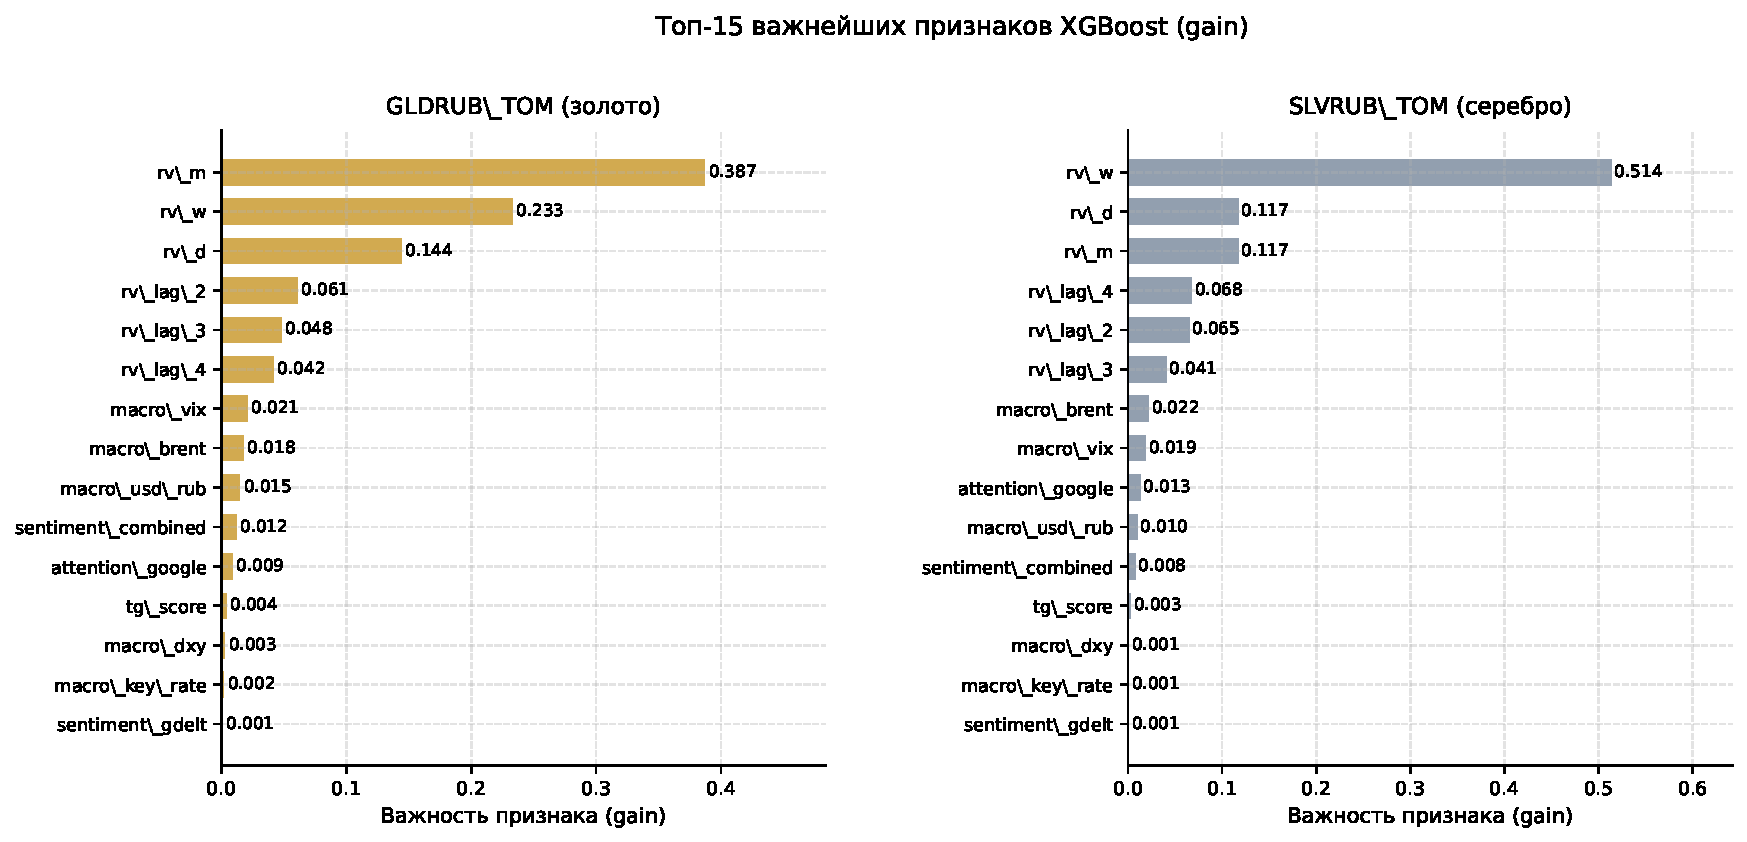
\includegraphics[width=\linewidth]{figures/feature_importance.pdf}
\caption{Важность признаков XGBoost (gain, нормировано).
         Слева~--- GLDRUB\_TOM (золото), справа~--- SLVRUB\_TOM (серебро).
         HAR-лаги доминируют; sentiment- и macro-признаки занимают нижние позиции.}
\label{fig:feature_importance}
\end{figure}

На рисунке~\ref{fig:xgb_forecast} показан прогноз модели XGBoost
в сравнении с фактическими значениями логарифмической реализованной волатильности
на тестовой выборке (40\% наблюдений).

\begin{figure}[H]
\centering
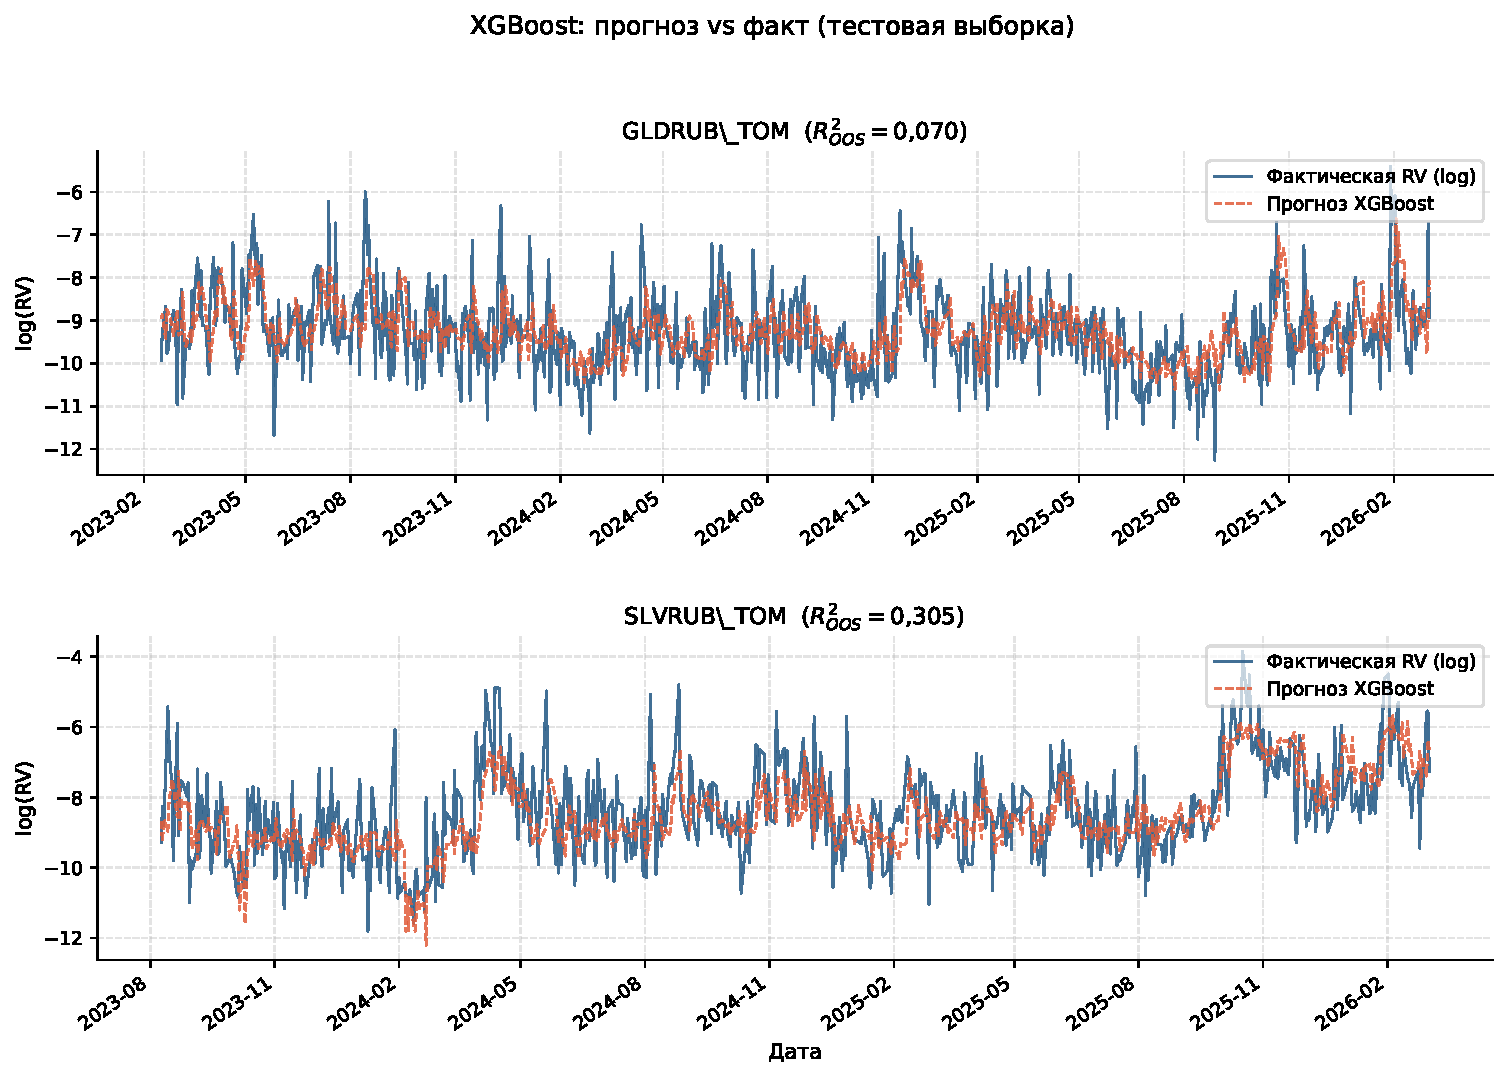
\includegraphics[width=\linewidth]{figures/xgb_forecast.pdf}
\caption{XGBoost: прогноз vs факт (log-RV) на тестовой выборке.
         Сверху~--- GLDRUB\_TOM, снизу~--- SLVRUB\_TOM.}
\label{fig:xgb_forecast}
\end{figure}

\subsection{Сравнительный анализ и тест Диболда--Мариано}
\label{sec:dm}

Сводные результаты всех моделей представлены в таблице~\ref{tab:full_results}.

\begin{table}[H]
\centering
\caption{Сравнение всех моделей (после фиксов: общая Patton QLIKE, лаг sentiment~1)}
\label{tab:full_results}
\begin{tabular}{llrrrr}
\hline
Инструмент & Модель & MAE & RMSE & $R^2_{\mathrm{OOS}}$ & QLIKE \\
\hline
GLDRUB\_TOM & HAR-log     & 0{,}674 & 0{,}869 & 0{,}177 & 0{,}628 \\
GLDRUB\_TOM & HAR-log-S   & \textbf{0{,}672} & \textbf{0{,}868} & \textbf{0{,}180} & \textbf{0{,}626} \\
GLDRUB\_TOM & XGBoost     & 0{,}725 & 0{,}924 & 0{,}070 & 0{,}627 \\
GLDRUB\_TOM & kNN ($k=75$)& 0{,}671 & 0{,}877 & 0{,}163 & 0{,}683 \\
\hline
SLVRUB\_TOM & HAR-log     & 0{,}838 & 1{,}060 & \textbf{0{,}377} & \textbf{0{,}979} \\
SLVRUB\_TOM & HAR-log-S   & 0{,}834 & 1{,}060 & 0{,}376 & 1{,}022 \\
SLVRUB\_TOM & XGBoost     & 0{,}879 & 1{,}119 & 0{,}305 & 1{,}237 \\
SLVRUB\_TOM & kNN ($k=30$)& 0{,}859 & 1{,}086 & 0{,}345 & 1{,}167 \\
\hline
\end{tabular}
\end{table}

Для оценки статистической значимости различий между моделями
применяется тест Диболда--Мариано~\cite{Diebold1995} с поправкой
HAC (Newey--West, ядро Бартлетта, $1$ лаг).
Тестируется нулевая гипотеза равенства ожидаемых функций потерь:
$H_0:\, \mathbb{E}[L(e_1) - L(e_2)] = 0$.
В таблице~\ref{tab:dm_test} приведены попарные результаты;
знак \textit{model1 better} означает, что первая модель имеет
статистически значимо меньшую функцию потерь.

\begin{table}[H]
\centering
\caption{Тест Диболда--Мариано: попарные сравнения моделей.
         {$^{***}p<0{,}01$; $^{**}p<0{,}05$; $^{*}p<0{,}10$}}
\label{tab:dm_test}
\small
\begin{tabular}{lllrrl}
\hline
Инструмент & Сравнение (M1 vs M2) & Потери & DM-статистика & $p$-value & Заключение \\
\hline
GLDRUB\_TOM & HAR-log vs HAR-log-S & SE     & $+0{,}97$  & $0{,}33$       & нет различий \\
GLDRUB\_TOM & HAR-log vs HAR-log-S & AE     & $+1{,}76$  & $0{,}08^{*}$   & M2 лучше \\
GLDRUB\_TOM & HAR-log vs HAR-log-S & QLIKE  & $+0{,}62$  & $0{,}53$       & нет различий \\
GLDRUB\_TOM & HAR-log vs kNN       & SE     & $-0{,}95$  & $0{,}34$       & нет различий \\
GLDRUB\_TOM & HAR-log vs kNN       & QLIKE  & $-2{,}41$  & $0{,}02^{**}$  & M1 лучше \\
GLDRUB\_TOM & HAR-log-S vs kNN     & QLIKE  & $-2{,}38$  & $0{,}02^{**}$  & M1 лучше \\
\hline
SLVRUB\_TOM & HAR-log vs HAR-log-S & SE     & $-0{,}13$  & $0{,}90$       & нет различий \\
SLVRUB\_TOM & HAR-log vs HAR-log-S & AE     & $+1{,}81$  & $0{,}07^{*}$   & M2 лучше \\
SLVRUB\_TOM & HAR-log vs HAR-log-S & QLIKE  & $-3{,}83$  & $<\!0{,}001^{***}$ & M1 лучше \\
SLVRUB\_TOM & HAR-log vs kNN       & SE     & $-1{,}83$  & $0{,}07^{*}$   & M1 лучше \\
SLVRUB\_TOM & HAR-log vs kNN       & QLIKE  & $-2{,}84$  & $0{,}005^{***}$& M1 лучше \\
SLVRUB\_TOM & HAR-log-S vs kNN     & AE     & $-2{,}04$  & $0{,}04^{**}$  & M1 лучше \\
SLVRUB\_TOM & HAR-log-S vs kNN     & QLIKE  & $-2{,}27$  & $0{,}02^{**}$  & M1 лучше \\
\hline
\end{tabular}
\end{table}

\subsection{Главные выводы}

\begin{enumerate}
    \item \textbf{Sentiment даёт ограниченный вклад.}
          Расширенный HAR-log-S c комбинированным sentiment-индексом
          улучшает MAE на обоих инструментах статистически значимо
          лишь на уровне 10\% ($p \approx 0{,}07$--$0{,}08$).
          По QLIKE улучшение наблюдается только на золоте и не значимо;
          на серебре sentiment даже \textit{ухудшает} QLIKE значимо ($p < 0{,}001$).
    \item \textbf{Лучший единичный sentiment-источник зависит от инструмента.}
          Для золота это взвешенный \texttt{sentiment\_combined},
          для серебра~--- \texttt{attention\_google} (Google Trends),
          что согласуется с теорией Да--Энгельберга--Гао о Google-индексе
          как самостоятельной мере внимания розничных инвесторов.
    \item \textbf{kNN не превосходит HAR после корректной настройки.}
          После унификации формулы QLIKE и устранения leakage по sentiment
          kNN(HAR+sentiment) проигрывает HAR-log/HAR-log-S по
          $R^2_{\mathrm{OOS}}$ и QLIKE на обоих инструментах;
          по MAE результат близок к ничьей.
          Полученный итог отличается от предыдущих внутренних расчётов
          по проекту, где kNN формально лидировал на золоте~---
          анализ источников расхождения (раздел~\ref{sec:dm}) показывает,
          что прежнее преимущество было артефактом несовместимых
          определений QLIKE и одновременности sentiment с целевой
          переменной.
    \item \textbf{XGBoost существенно уступает HAR.}
          Это типично для задач прогнозирования волатильности
          дневной частоты: нелинейное усложнение модели
          не компенсирует шум множества дополнительных признаков
          при ограниченном размере выборки.
\end{enumerate}

\subsection{Ограничения и направления развития}

Текущие результаты получены при частично заполненном sentiment-векторе:
данные GDELT охватывают $\approx$\,718 дней с ненулевым покрытием
(остальные дни заполнены методом forward fill),
NLP-агрегация RSS-новостей даёт устойчиво нулевой sentiment для
большинства дней, что объясняет нулевой вклад этого источника в ablation
(таблица~\ref{tab:har_ablation}).
Расширение NLP-покрытия RSS, увеличение Telegram-архива
до сопоставимой плотности и подключение дополнительных макро-сигналов
(данные ЦБ РФ по объёмам сделок СВОП, индексы геополитической
неопределённости~GPR) являются естественными направлениями
дальнейшей работы.
